\chapter{Pandas}
\section{Introduction to Pandas}
Pandas is a popular python library for dealing with database. It is one of our primary tool in this course. Let us first import Pandas.

\begin{figure}[ht]
	\centering
	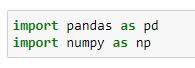
\includegraphics{Assets/Images/Pandas/import}
	\caption{Importing Pandas as pd}
	\label{fig:import}
\end{figure}

\noindent We would then load our dataset and import them as Pandas dataset.

\begin{figure}[ht]
	\centering
	\includegraphics[width=1.0\linewidth]{"Assets/Images/Pandas/read data"}
	\caption{Importing data}
	\label{fig:read-data}
\end{figure}

\noindent We can simply call the data by typing it's name (in this case \textit{drug}).
\begin{figure}[ht]
	\centering
	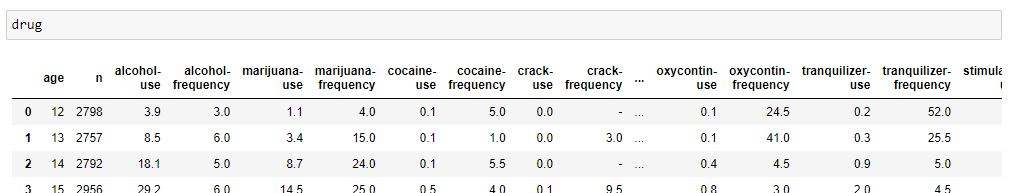
\includegraphics[width=1\linewidth]{Assets/Images/Pandas/drugs}
	\caption{Calling the data}
	\label{fig:drugs}
\end{figure}

\noindent If we only want to see the first few rows, we use the \textit{head} method. Which is 5 by default.

\begin{figure}[ht]
	\centering
	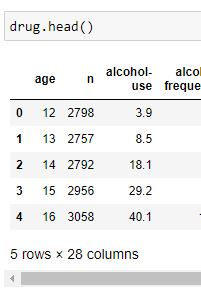
\includegraphics{Assets/Images/Pandas/head}
	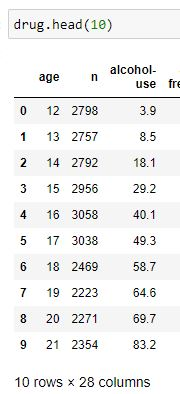
\includegraphics{Assets/Images/Pandas/head10}
	\caption{Using head method}
	\label{fig:head}
\end{figure}

\noindent Likewise, the \textit{tail} method for last few rows.

\begin{figure}[ht]
	\centering
	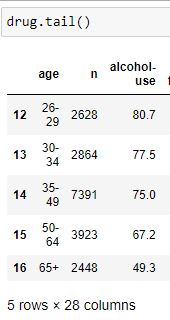
\includegraphics{Assets/Images/Pandas/tail}
	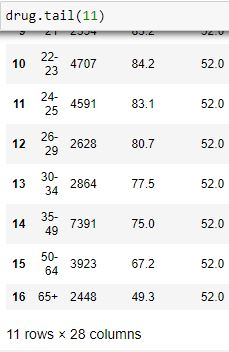
\includegraphics{Assets/Images/Pandas/tail11}
	\caption{Using tail method}
	\label{fig:tail}
\end{figure}

\newpage
\noindent The \textit{index} method is used to examine index which could be handy to detect duplicates

\begin{figure}[ht]
	\centering
	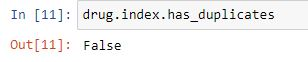
\includegraphics{Assets/Images/Pandas/index_duplicates}
	\caption{Using index method}
	\label{fig:index}
\end{figure}

\noindent We can use \textit{shape} method to examine the dimensions of our data.

\begin{figure}[ht]
	\centering
	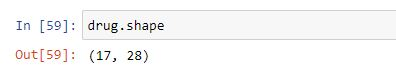
\includegraphics{Assets/Images/Pandas/shape}
	\caption{Using shape method}
	\label{fig:index}
\end{figure}
\section{EDA and Data Cleaning}
\section{Grouping}